In this section, we present the architecture and implementation of a system that monitors the status of multiple nodes via serial communication and displays their status in a graphical user interface. The system consists of two main components:
\begin{itemize}
    \item A background thread that reads and processes incoming serial data.
    \item A user interface that visualizes node states in real-time using colored labels.
\end{itemize}

\subsection{Reading from the Serial}

The serial communication is handled by the \texttt{SerialReaderThread} class, which runs in a background thread to avoid blocking the GUI. Its main functionality is found in the \texttt{read\_serial()} method. The thread checks if data is available (\texttt{in\_waiting > 0}), reads and decodes the incoming string, and logs it. If the message follows the format \texttt{Node<id> - State:<STATE>}, the node ID and state are extracted. This call delegates the responsibility of updating the GUI to the main application \texttt{HydrotrackerMonitor}.

\subsection{Data Processing}
Once a valid line is received, the data is parsed into two components:
\begin{itemize}
    \item \texttt{node\_id}: the identifier of the node
    \item \texttt{state}: the reported status (e.g., "EMPTY", "NOTEMPTY", or "NOTEXIST")
\end{itemize}
After extracting these, the GUI is updated only if the state has changed. Each node has an entry in a dictionary \texttt{node\_states} that keeps track of its most recent state. This structure allows for efficient updates and state comparisons.

\subsection{User Interface}
The GUI is created using Python's \texttt{tkinter} module and is managed by the \texttt{HydrotrackerMonitor} class. For each detected node, a label is dynamically added with the method \texttt{create\_gui\_label(node\_id)}. Each label changes its color and text based on the node's current state. This is managed in the \texttt{update\_gui\_loop()} method, which periodically refreshes the display.

\begin{figure}[H]
    \centering
    \begin{subfigure}[b]{0.45\linewidth}
        \centering
        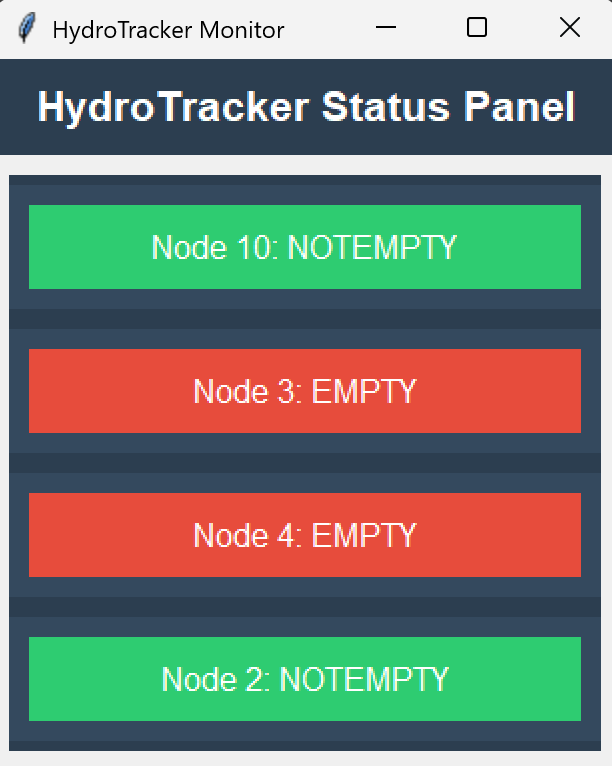
\includegraphics[width=\linewidth]{gui_images/gui_screenshot_1.png}
        \caption{}
        \label{fig:subfig1}
    \end{subfigure}
    \hfill
    \begin{subfigure}[b]{0.45\linewidth}
        \centering
        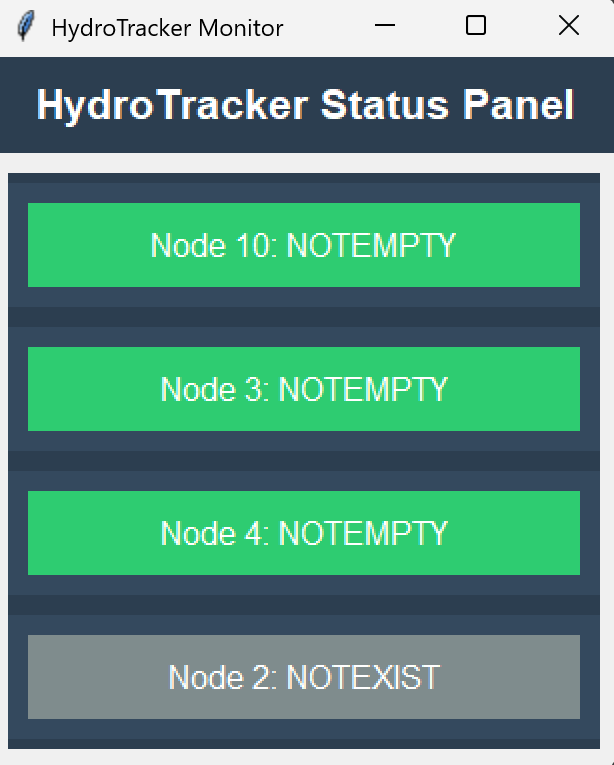
\includegraphics[width=\linewidth]{gui_images/gui_screenshot_2.png}
        \caption{Caption for second image}
        \label{fig:subfig2}
    \end{subfigure}
    \caption{}
    \label{fig:combined}
\end{figure}